\chapter{Laajempi esimerkki}\label{esimerkki}

Tarkastellaan vielä lopuksi laajempaa esimerkkiä. Tarkastellaan normaalia lineaarista regressiomallia. Käytetään \texttt{R}:stä löytyvää \texttt{airquality} aineistoa New Yorkin ilmanlaadusta. Sovitetaan aineistoon bayesilainen lineaarinen malli
\begin{equation}
	\texttt{Ozone} = \beta_0 + \beta_1\texttt{Solar.R} + \beta_2\texttt{Wind}
\end{equation}
 Gibbsin otanta-algoritmin avulla. 

Määritellään ensiksi malli. Merkitään $\tau = 1/\sigma^2$, $\theta = (\beta_0,\beta_1,\beta_2,\tau)$ ja asetetaan \emph{prioirijakaumat} \emph{konjugaattijakaumiksi}.
\begin{equation}
\begin{split}
	y_i|\beta_0,\beta_1,\beta_2,\tau &\sim N(\beta_0+\beta_1 x_i+\beta_2x_i, 1/\tau) \\
	\beta_0|\mu_0,\tau_0 &\sim N(\mu_0, 1/\tau_0) \\
	\beta_1|\mu_1,\tau_1 &\sim N(\mu_1, 1/\tau_1) \\
	\beta_2|\mu_2,\tau_2 &\sim N(\mu_2, 1/\tau_2) \\
	\tau|\alpha, \gamma &\sim \mathrm{Gamma}(\alpha, \gamma)
\end{split}	
\end{equation}
Muodostetaan uskottavuusfunktio
\begin{equation}
	L(y|\theta) = \prod_{i=1}^{N} N(\beta_0+\beta_1 x_i+\beta_2x_i, 1/\tau)
\end{equation}
Posterioirijakauman tiheysfunktio on siten laskettavissa verrannollisuudella
\begin{equation}
	p(\theta|y) \propto p(\beta_0)p(\beta_1)p(\beta_2)p(\tau)\prod_{i=1}^{N} N(\beta_0+\beta_1 x_i+\beta_2x_i, 1/\tau)
\end{equation}
Tästä saadaan sitten johdettua ehdolliset jakaumat otanta-algoritmia varten
\begin{equation}\label{marginaalit}
\begin{split}
	\beta_0 | \beta_1,\beta_2,\tau_0,\tau,\mu_0,x,y &\sim 
	N\pqty{\frac{\tau_0\mu_0+\tau\sum_{i=1}^{N}(y_i-\beta_1x_{i1}-\beta_2x_{i2})}{\tau_0+\tau N}, \frac{1}{\tau_0+\tau N}} \\
	\beta_1 | \beta_0,\beta_2,\tau_1,\tau,\mu_1,x,y &\sim 
	N\pqty{\frac{\tau_1\mu_1+\tau\sum_{i=1}^{N}(y_i-\beta_0-\beta_2x_{i2})x_{i1}}{\tau_1+\tau\sum_{i=1}^{N}x_{i1}^2}, \frac{1}{\tau_1+\tau\sum_{i=1}^{N}x_{i1}^2}}\\
	\beta_2 | \beta_0,\beta_1,\tau_2,\tau,\mu_2,x,y &\sim 
	N\pqty{\frac{\tau_2\mu_2+\tau\sum_{i=1}^{N}(y_i-\beta_0-\beta_1x_{i1})x_{i2}}{\tau_2+\tau\sum_{i=1}^{N}x_{i2}^2}, \frac{1}{\tau_2+\tau\sum_{i=1}^{N}x_{i2}^2}}\\
	\tau | \beta_0,\beta_1,\beta_2,\alpha,\gamma,x,y &\sim 
	\mathrm{Gamma}\pqty{\alpha+\frac{N}{2},\gamma + \frac{N}{2}\sum_{i=1}^{N}(y_i-\beta_0-\beta_1x_{i1}-\beta_2x_{i2})^2}
\end{split}
\end{equation}
Asetetaan hyperparametrit $\mu_0 = 80,\mu_1 = 0, \mu_2 = -5, \tau_0 = 1/50, \tau_1 = 1/50, \tau_2 = 1/50, \alpha	= 5, \gamma = 0.01$. Parametrit on valittu sen mukaan, että ne asettavat jakauman moodin lähelle arvioitua sijaintia ja toisaalta eivät ole kovin informatiivisia vaan paksu häntäisiä. Simuloidaan nyt tästä Gibbsin otanta-algoritmilla yhtälöitä \ref{marginaalit} käyttäen 8 ketjua, kunkin pituus 2 000. Burnin-periodi olkoot 1 000. Yhteensä siis meillä on  16 000 otosta, joista 8 000 leikataan pois ja 8 000 jätetään arvioitavaksi.

% latex table generated in R 3.6.1 by xtable 1.8-4 package
% Tue Apr  7 16:14:05 2020
\begin{table}[ht]
\centering
\label{results}
\begin{tabular}{rrrrrrrr}
  \hline
 $\theta$ & Mean & SD & 2.5\% & 25\% & 50\% & 75\% & 97.5\% \\ 
  \hline
  $\beta_0$ & 78.89544 & 5.61842 & 67.97969 & 75.14744 & 78.89385 & 82.64874 & 89.86483 \\ 
  $\beta_1$ & 0.09675 & 0.02263 & 0.05196 & 0.08130 & 0.09688 & 0.11218 & 0.14106 \\ 
  $\beta_2$ & -5.48880 & 0.51291 & -6.48407 & -5.83627 & -5.49158 & -5.13095 & -4.48973 \\ 
  $\tau$ & 0.00177 & 0.00023 & 0.00136 & 0.00161 & 0.00176 & 0.00192 & 0.00226 \\ 
   \hline
\end{tabular}
\caption{Tulokset regressiosta}
\end{table}
\begin{table}[ht]\label{diagnostics}
\centering
\begin{tabular}{rrr}
  \hline
 $\theta$ & $\hat{R}$ & $\hat{n}_{\mathrm{eff}}$ \\ 
  \hline
  $\beta_0$ & 1.00 & 778 \\ 
  $\beta_1$ & 1.00 & 1177 \\ 
  $\beta_2$ & 1.01 & 902  \\ 
  $\tau$ & 1.00 & 7656  \\ 
   \hline
\end{tabular}
\caption{Diagnostiikka}
\end{table}

Taulukoissa 4.1 ja 4.2 nähdään tulokset ja MCMC-diagnostiikat, joista puhuttiin aiemmin. Nähdään, että ketjut näyttäisivät konvergoituneen, mikä ei sinänsä ihmetytä, sillä simulaatio määrämme on suurehko.

Mielenkiintoista on nähdä, että kuvassa \ref{kuva1} ketju parametrille $1/\tau$ on aivan erinäköinen kuin muille parametreille. Otoksia on yhtä paljon kaikissa, mutta parametrin $1/\tau$ ketju näyttää siltä, että otoksia olisi enemmän. Tämä nähdään myös $\hat{n}_{\mathrm{eff}}$ estimaatista.

\begin{figure}[h!]
	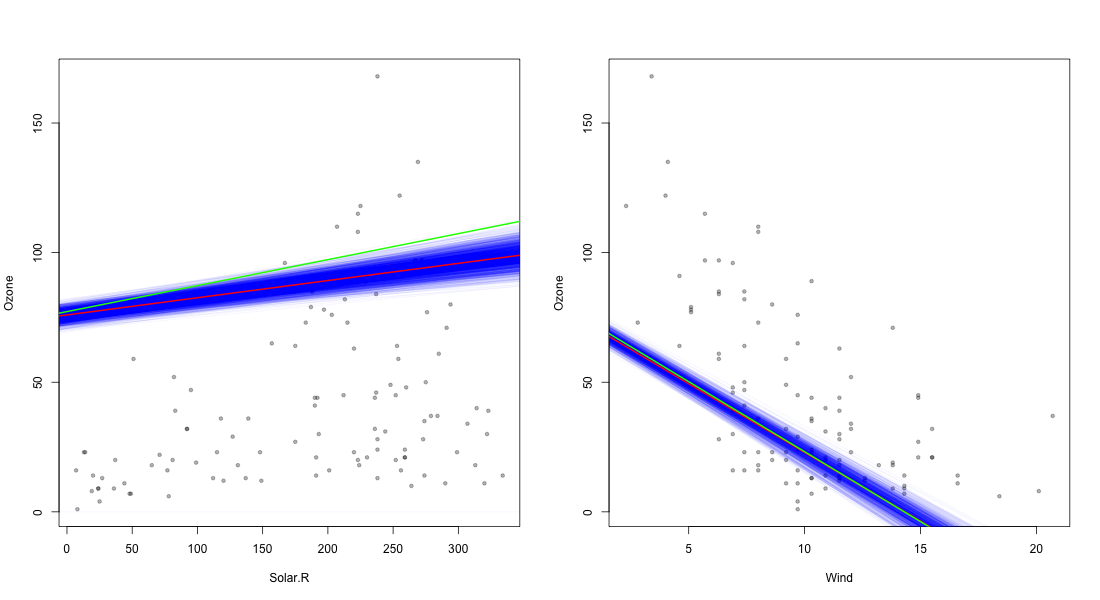
\includegraphics[width=\textwidth]{gibbsexample}
	\caption[Regressio]{\textit{Esimerkin lineaarisen regression tulos, vasemmalla Solar.R $x$-akselilla ja oikealla Wind. Punainen viiva on posteriori odotusarvolla piiretty regressioviiva ja vihreä on vertailun vuoksi PNS-mentelmällä sovitettu suora. Siniset ovat sovitteita parametrien eri ehdotusarvoilla.}}
	\label{kuva1}
\end{figure}

\begin{figure}[h!]
	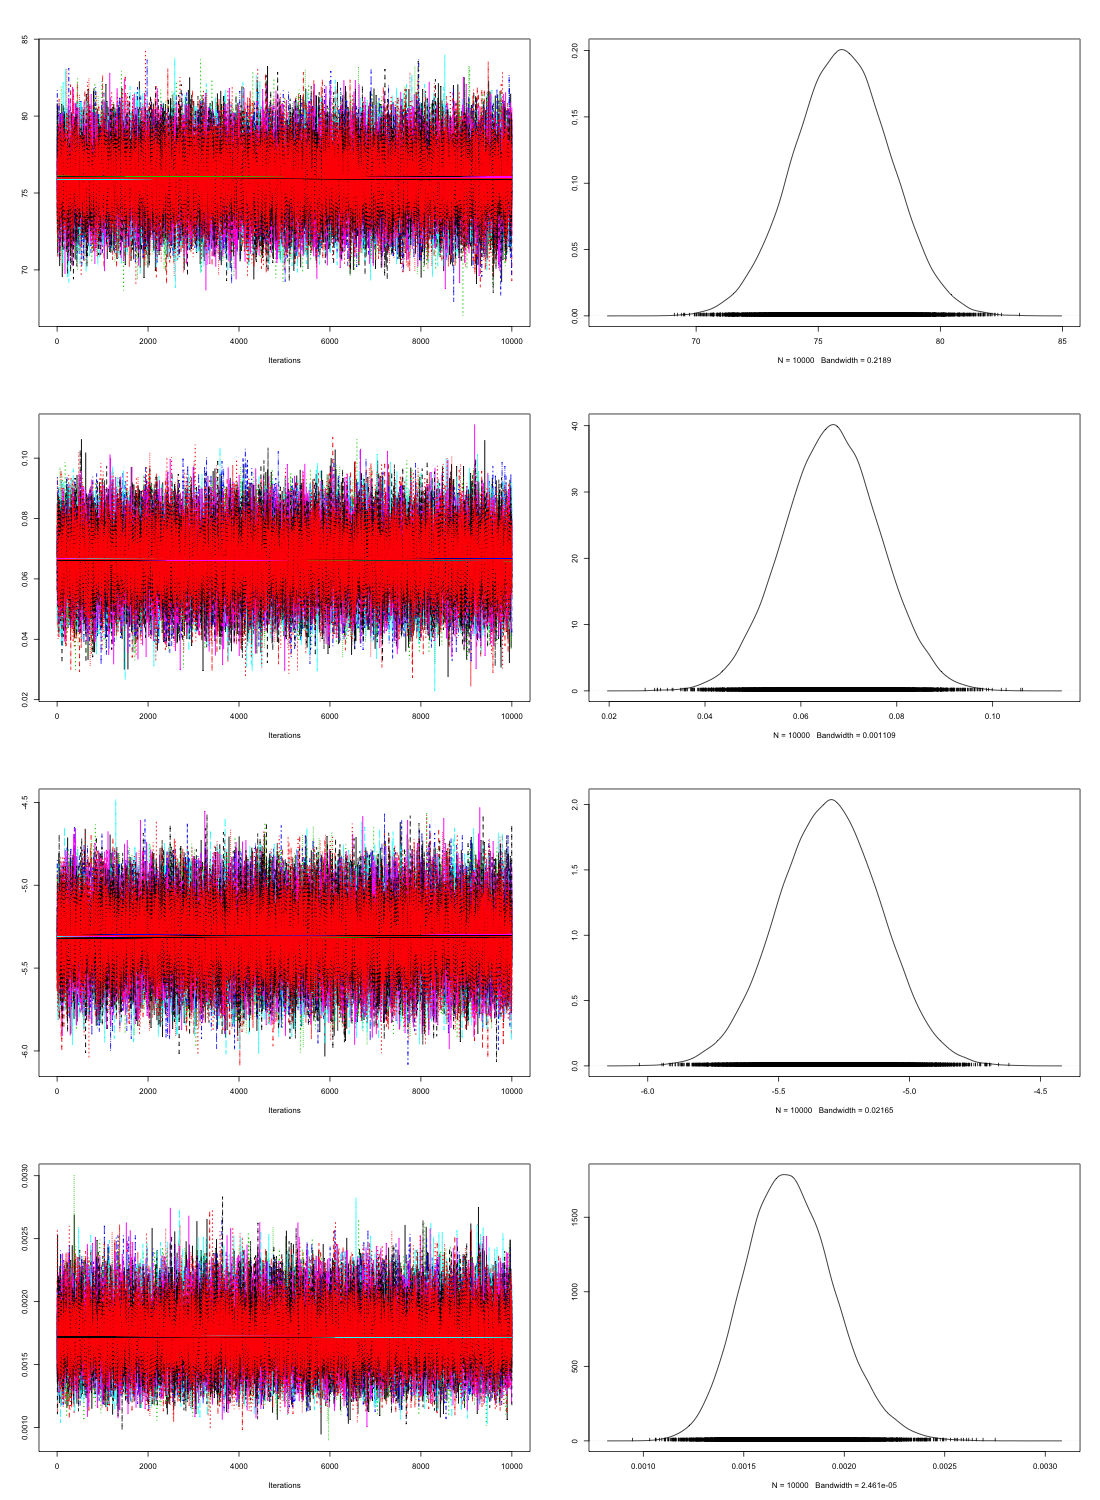
\includegraphics[width=\textwidth]{gibbs2}
	\caption[]{\textit{Esimerkin ketjut ja parametrien posteriori tiheydet}}
	\label{kuva1}
\end{figure}



